\documentclass[a4paper,14pt,russian]{extreport}
\usepackage[russian]{babel}

\usepackage{../common/dsturep_ru} % оформление по ДСТУ 3008-95
\usepackage{import}
\usepackage{standalone}
\usepackage{comment}
\usepackage{bbm}

\usepackage{tikz}
\usepackage{tikz-3dplot}
\usetikzlibrary{calc}
\usetikzlibrary{plotmarks}
\usepackage{pgfplots}

%\usepackage{scrextend}
\usepackage{changepage}
\usepackage{caption}
\usepackage{listings}
%\usepackage[title,titletoc]{appendix}
%\usepackage{appendix}
\usepackage{longtable}
%\usepackage{slashbox}
\usepackage{diagbox}
\usepackage{lscape}
\usepackage{algorithmic}
\usepackage{algorithm}

\def\male{male}
\def\female{female}

\bibliographystyle{../common/utf8gost780u}

\usepackage[square,numbers,sort&compress]{natbib}
\renewcommand{\bibnumfmt}[1]{#1.\hfill} % нумерация источников в самом списке — через точку

\def\passYear{2017}
\def\faculty{физико-технический институт}
\def\department{Кафедра информационной безопасности}
\def\departmentHead{Н. В. Грайворонский}
\def\kind{Дипломна робота}
\def\level{магістр}
\def\specialityCode{8.04030101}
\def\specialityTitle{Прикладная математика}
\def\theme{Решение нелинейных уравнений}
\def\gender{female}
\def\mentorGender{male}
\def\course{3}
\def\group{ФИ-41}
\def\name{Лавягина Ольга Алексеевна}
\def\mentorRank{}
\def\mentorName{Стёпочкина Ирина Валерьевна}
\def\reviewerRank{Rank}
\def\reviewerName{Name}
\def\subject{Методы вычислений}



\begin{document}

\import{1_title/}{title.tex}

\clearpage

\pagenumbering{gobble}
%\import{3_abstract/}{main.tex}

%\pagestyle{empty}
%\thispagestyle{empty}
%\tableofcontents

\clearpage
\pagenumbering{arabic}
\pagestyle{fancy}
\setcounter{page}{2}

\clearpage

\chapter{Исходные данные}

В компьютерном практикуме (вариант 8) ищутся корни уравнения
\begin{equation} \label{eq:1}
2x^5 + 3x^2 - 2x - 6 = 0.
\end{equation}

\chapter{Допрограммный этап}

Корни уравнения были найдены с помощью \href{http://www.wolframalpha.com}{WolframAlpha}, построен график (рис. \ref{fig:plot}).

\begin{figure}[h!]
  \centering
  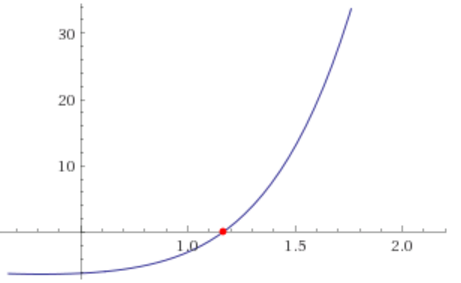
\includegraphics[width=.3\textwidth]{plot.png}
  \caption{График полинома $f \left( x \right) = 2x^5 + 3x^2 - 2x - 6$}
\label{fig:plot}
\end{figure}

Красной точкой на графике отмечен корень уравнения \ref{eq:1}.
Он лежит на промежутке от $1$ до $1.5$.

\chapter{Листинг программы}

Листинг файла utils.py
\lstset{inputencoding=utf8, extendedchars=\true}
\lstinputlisting[language=python,
                 basicstyle=\ttfamily\scriptsize]{../code/utils.py}

Листинг программы уточнения корней по методу бисекции
\lstset{inputencoding=utf8, extendedchars=\true}
\lstinputlisting[language=python,
                 basicstyle=\ttfamily\scriptsize]{../code/bisection.py}

Листинг программы уточнения корней по методу хорд
\lstset{inputencoding=utf8, extendedchars=\true}
\lstinputlisting[language=python,
                 basicstyle=\ttfamily\scriptsize]{../code/horde.py}

Листинг программы уточнения корней по методу Ньютона (касательных)
\lstset{inputencoding=utf8, extendedchars=\true}
\lstinputlisting[language=python,
                 basicstyle=\ttfamily\scriptsize]{../code/newton.py}

\chapter{Результаты работы программы}

Результаты метода бисекции
\lstset{inputencoding=utf8, extendedchars=\true}
\lstinputlisting[language=bash,
                 basicstyle=\ttfamily\scriptsize]{../code/bisection_result.txt}

Результаты метода хорд с критерием завершения процесса $ \left| f \left( c \right) \right| < \varepsilon $
\lstset{inputencoding=utf8, extendedchars=\true}
\lstinputlisting[language=bash,
                 basicstyle=\ttfamily\scriptsize]{../code/horde_result.txt}

Результаты метода хорд с критерием завершения процесса
$$\left| c - c_{previous} \right| < \varepsilon $$
\lstset{inputencoding=utf8, extendedchars=\true}
\lstinputlisting[language=bash,
                 basicstyle=\ttfamily\scriptsize]{../code/horde_result_difference.txt}

Результаты метода Ньютона (касательных)
\lstset{inputencoding=utf8, extendedchars=\true}
\lstinputlisting[language=bash,
                 basicstyle=\ttfamily\scriptsize]{../code/newton_result.txt}

\chapter*{Выводы}
\addcontentsline{toc}{chapter}{Выводы}

С помощью метода бисекции корень заданного уравнения был получен на 16-й итерации,
с помощью метода хорд --- на 13-й,
а с помощью метода Ньютона (касательных) ---на четвёртой.

Для метода бисекции было обнаружено, что при увеличении длины отрезка количество итераций возрастает, но при уменьшении длины отрезка практически не меняется.
Так, для отрезка $ \left[ 1.1, 1.2 \right] $ результат был получен на 14-й итерации.

Метод хорд даёт результат гораздо быстрее.
Для отрезка $ \left[ 1.1, 1.2 \right] $ результат был получен за на четвёртой итерации.

Преимуществом метода Ньютона (касательных) является его быстрая сходимость.
Для данного метода необходимо знать начальное приближение, а не границы интервала, в котором находится корень.
Недостатком является то, что метод может зацикливаться (в данном случае, например, при $x_0 = 1$).

\end{document}
